\section{Introduction}
This paper is about an academic project born to be an efficient solution for the CINI\footnote{Consorzio Interuniversitario Nazionale per l'Informatica} 2017 Challenge on smart cities illumination systems. In particular, the goal was to prototype and test a solution which was capable of (near) real-time data stream processing for monitoring records from street lamps, lumen sensors co-located with the street lamp itself and from traffic data produced by third-party APIs. We will explore this solution for the following use case: in a smart city context it is necessary to guarantee the maximum efficiency from lamps consumption while providing an optimal illumination within safety limits for pedestrians and drivers and according to local traffic intensity. To achieve that, it is necessary to project a grid of smart lamps capable of tuning their light level according to the right amount of energy necessary to provide city aware, safe and green consumption levels. This grid must be powered and managed via a reliable, highly available, processing-capable control system. Introducing Project Ember.


\section{Frameworks and Tools}
We structured our environment using at first a publish/subscribe architecture with street lamps, lumen and traffic sensors as publishers and the stream processing framework as subscriber. 

\subsection{Data stream processing}
The Apache Software Foundation makes available different alternatives, each one a refined version of the previous: Apache Storm is one of the most used data stream processing framework on the market and one of the most supported as well; Apache Spark is a refined version of Storm even though it is limited to fewer programming languages (Java, Scala and Python); Apache Flink\footnote{Apache Flink official page: https://flink.apache.org/} is the most recent project among the three and the most advanced. Flink gives the programmer the possibility to define just the topology of the operators, how they are linked, or how to set the windows timing (based upon the event time or upon the processing time spent inside the system). Flink handles the under-the-hood engine: multithreading, synchronization, parallelism, availability, cluster management. We chose the latest stable release of Apache Flink, 1.2.0, which comes with a well written documentation as well as multiple connectors for the most popular MOM\footnote{Messages Oriented Middleware} and storages. Flink calls a Source the very component that produces data and Sink the one that takes the processed data in order to store or to route them to another entity.

\subsection{Connectors}
To achieve scalability we had to analyze several options to let connect our Flink topology to messages routers and to the persistence level. The MOM chosen was Apache Kafka\footnote{Apache Kafka documentation: https://kafka.apache.org/documentation} works seamlessly with Flink thanks to the included connector plugins giving the possibility to simply personalize the connection according to our preferences: in particular in this solution Kafka is our preferred Source to handle data from the sensors. Talking about the Sinks, Flink supports many platforms and Kafka can be one of them (for example for the control output), but in order to persist and manage our data we wanted to use also a modern platform capable of organizing data for (near) real-time purposes.

\subsection{Persistence level}
A NoSQL approach was mandatory to us, to collect dynamic unstructured data typical of a sensor network, so we analyzed different products: in particular Elasticsearch\footnote{Elasticsearch official page: https://www.elastic.co/products/elasticsearch} and Apache Cassandra. We chose Elasticsearch, as it is fully supported (not its last version indeed) by Flink 1.2.0 and it is a flexible, easy-to-deploy database with RESTful APIs. It leverage the ability to perform complex queries, even geographical and lexical ones, with good performances and scalability options. Elasticsearch is part of the Elastic Stack built by Elastic.co which makes available another useful tool for visualizing data stored in Elasticsearch, Kibana\footnote{Kibana official page: https://www.elastic.co/products/kibana}.

\subsection{Extras}
To develp a local control unit to manage the city grid we used Flask and Redis. Flask\footnote{Flask official page: http://flask.pocoo.org/} is a micro-framework for Web Server built in Python and Redis\footnote{Redis official page: https://redis.io/} instead is simple and efficienty key-valye data store and works as a database, cache and message broker. Redis serves us as a cache, allowing us to interact with control unit history with it with very simple APIs via the endpoints exposed by Flask.

\subsection{Programming languages}
Java is the programming language that links all these components together being used by Flink as well as Scala, such as Elasticsearch APIs. We also used Python for the control unit development as well as to realize the simulated data source for testing.


\section{Architecture overview}
In this section we will cover how the system communicates between each of its components and modules and the assumptions we made to prototype and test the architecture. In \hyperref[fig:ember_architecture]{figure 1} a high-level architecture overview is provided. Before proceeding, we want to focus on the output from the real-time\footnote{We will define the system as "real-time" in this paper even if is not validated for such a control system, but it is capable of near real-time data streams processing} control system: it is produced into the MOM and consumed by control units (how will be discussed later), closing a feedback loop. This behavior and the capabilities to maintain high-availability across the clusters make the system itself near to the features of an autonomic system.
\begin{figure}[!b]
\begin{center}
	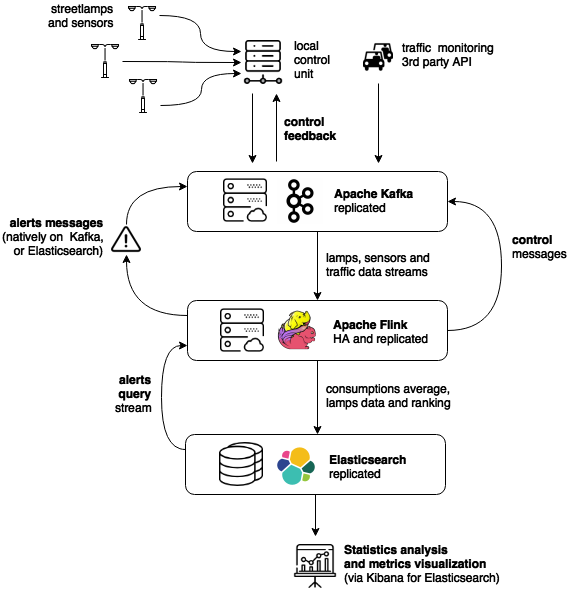
\includegraphics[scale=0.35]{img/ember_architecture}
	\caption{Project Ember architecture overview}
	\label{fig:ember_architecture}
\end{center}
\end{figure}

\subsection{Sensors network}
First of all let us consider how the sensors network sends its data to the control system. According to project specifications the street lamps sends to the system a JSON formatted string containing all the information their microcontrollers collect as a tuple\footnote{in particular a unique integer id, address and model, consumption, intensity level, power on status and last replacement (as a timestamp in seconds) plus the timestamps in seconds of the instant the tuple was sent}. Those data are sent every 10 seconds. A lumen sensor is placed on the lamp and it sent data with same rate as well giving us information about the daylight luminosity level and the id of the lamps it is placed upon.

\subsection{Control unit}
The control unit gives us the possibility to create a new indirection level that is placed among the lamps and Flink. The lamps talk, using the city intranet, to the local control unit which maintains a mapping between the lamps ids and their IP addresses inside the local city network. The control unit manage the correct routing of the messages from the lamps to the stream processing operator via Kafka, as well as the control feedback received via the same MOM. This solution was introduced both for the indirection it introduces and the plug-and-play registration of each new lamp via RESTful APIs, as well as the capability to store the sensible data at the edge of the network to decrease latency, giving us some features of the fog computing paradigm.

\subsection{Apache Kafka cluster}
To handle the thousands of data necessary to manage the infrastructure, we thought to use a cluster of replicated nodes running the same Apache Kafka instance, using Apache Zookeeper\footnote{Apache Zookeeper official page: https://zookeper.apache.org} to maintain the cluster available via redirection from a public IP. As we will see later, the MOM allows us to register topics for lamps, sensors and traffic monitoring data to retrieve them as a stream in Flink, and to create automatically topics for each control unit in order to retrieve the control feedback for each sector of the city grid. In addiction we included the possibility to route via Kafka alerts messages (to be consumed later by a custom operator).

\subsection{Apache Flink cluster}
This is the core of the architecture. The Apache Flink framework was used to create a data stream (near) real-time processing system to handle the thousands of tuples per seconds from the city grid and to produce for each of them a control output, as well as aggregations by streets or identifiers to produce statistics, ranks (by last replacement) and to store them for further analysis. Flink is also used to continuously monitor data from Elasticsearch and to produce alerts for any kind of failures that is collectable from each lamp history. To provide the necessary resilience and to let the processing system to scale, it is intended to be deployed as an highly-available cluster, composed of a JobManager (replicated and managed via Apache Zookeeper), acting as a master, and some TaskManagers, acting as slaves, into which is replicated every stream according their computational power (one core is one execution slot), producing several degrees of parallelism proportional to the cluster size. Moreover, it is handled via the JobManager any transition from a set of parallelized stream into a single time window to perform any bath computation (as for example average computation).

\subsection{Elasticsearch and Analytics}
The ranks, the consumption mean by id and by address, have to be visualized and showed in real-time, so Elasticsearch comes in help. Flink offers an interface for Elasticsearch, that, simply providing the cluster configuration, connects to it and allows to send data in byte encoded json format strings. Elasticsearch organizes data by so called Indexes and Types. The Index is the equivalent of Database in a NoSQL approach and the Types the equivalent of Tables. Elasticsearch keeps tracks of data assigning them a mapping table so it can be capable of understand primitives or complex data types. Kibana comes in our help for representing them. By a simple file of configuration you can use Kibana to create your own dashboard by defining all the data to be analyzed specifying the Type it has to use, how rearrange the attributes, how to order and in which style visualize them. Elasticsearch and Kibana has been designed to easily interact each other, keeping synchronized the dashboard across Kibana clients, and be simply deployed as well. Elasticsearch can be extended without any amount of effort, simply defining new nodes for the cluster and joining the master node. Elasticsearch serves also a particular role: being designed as a RESTful engine as well, it allows to specify complex query and resolves them efficiently, using at its core Apache Lucene, an open source machine learning library.


\section{DATA STREAM PROCESSING}


\section{A Message oriented approach}
Apache Kafka plays its MOM role connecting all the components of our system so let’s see how they are related to each other thanks to it: control units and Flink produce a lot of data in streams that are organized in topics: lamps, lumens and traffic, being specific. A system such as this can be sufficient but let’s think: being a smart lamps grid the system has to emit orders directed to a single lamp among thousands. Kafka can manage runtime topics creation but a topic for each lamp is meaningless and inefficient; requiring the data stream processing system to know the right position of the lamp among network is infeasible as well. Let we analyze better the problem.

% TODO insert image of kafka routing topology!

\subsection{Sensors to Kafka}
Lamps are supposed to be given, with a micro-controller built inside them capable to connect to the city intranet, to understand the power level proper of the bulb model and how such parameters relates one another in order to obtain the right luminosity. A lamp produce a JSON formatted string containing: the lamp id, the model of the light bulb, the timestamp of the last replacement instant of time, the current power consumption, the luminosity level, the control unit where it is registered, etc.

The lumen sensor is placed upon the street lamp and is managed by the same micro-controller; lumen sensors common for entire streets are managed as well. The lumen produce a JSON formatted string containing the same id of the lamp where it is placed upon (or a nonce for the common sensors), the luminosity value recorded, the street where it is located and the timestamp of the time instant when the data has been recorded.

The traffic sensor is realized by third party APIs and it is registered to Kafka producing a JSON formatted string containing the street monitored, the traffic value and the timestamp of the recorded time.

\subsection{Kafka to Adapters}
Once Flink calculates the state a street lamp should have it sends control directives to custom topics. Each lamps, in fact, is linked to a control unit and this information is included in the JSON sent by lamps to the system. That’s where the control directive is routed, a topic that is identified by the string that identify the control unit responsible of a particular street lamp; so we can, on one hand, free Kafka of an incredible number of topics and, on the other hand, free smart lamps to register themselves on their ones. As we said even the alerts of lamps not functioning or not communicating for a too long time can be routed to Kafka. Such alarms are simply transmitted to it using the connector provided by Flink that requires a byte encoding of the Alert object and the specification of the topic where they are directed to, a custom module can be easily engineered via a Kafka consumer to handle the alerts properly (our project let the user specify via configuration file to store the alerts into Elasticsearch instead).

\subsection{Controlling the lamps}
Each lamps is registered to a particular control unit (we will cover how in the next section), which takes care to register itself to the topic of its own, so it can read the responses and understands to which lamp direct them. Once the response will be made available the control unit reads the messages and convert them to a JSON object so it can access their attributes; it determines the id of the lamp and check in the Redis database to find the IP address related to that lamp id. That’s the core of the indirection level of the whole architecture. Kafka and the control unit makes possible all of this, making our system totally plug and play for a better large scale deployment.


\section{THE CITY GRID}

\subsection{Local streetlamps control}
%We needed a web server component capable of directing lamps data to Kafka and directive from Flink to lamps. The control unit has been built with such purpose in mind giving us the possibility to create a new indirection level that is placed among lamps and Kafka/Flink. Lamps talks to the control unit which maintains a mapping between the lamps IDs and their IP addresses inside the local city network. Lamps have to be registered to the right control unit in order to submit their data inside the system which increases the security level of our system (once placed, the lamp has to be registered by the local control unit, which could manage a street or a district; such operation needs to be done by an operator that places the lamp). The control unit validates the lamps and sends their data to the Kafka lamp topic. 
\subsection{Control units at scale}


\section{TESTS AND PERFORMANCES}

\subsection{The city simulator}


\section{NEXT STEPS AND CONCLUSIONS}

\subsection{Security}

\subsection{Deployment}

\subsection{Conclusions}


% to insert a simple bar chart
%\begin{tikzpicture}
%\begin{axis}[
%	x tick label style={
%		/pgf/number format/1000 sep=},
%	ylabel=Year,
%	enlargelimits=0.05,
%	legend style={at={(0.5,-0.1)},
%	anchor=north,legend columns=-1},
%	ybar interval=0.7,
%]
%\addplot 
%	coordinates {(2012,408184) (2011,408348)
%		 (2010,414870) (2009,412156) (2008,415 838)};
%\addplot 
%	coordinates {(2012,388950) (2011,393007) 
%		(2010,398449) (2009,395972) (2008,398866)};
%\legend{Men,Women}
%\end{axis}
%\end{tikzpicture}